\documentclass[11pt]{article}
\usepackage[letterpaper,margin=0.83in,headheight=16pt]{geometry}
\usepackage[T1]{fontenc}
\usepackage[utf8]{inputenc}
\usepackage{lmodern}
\usepackage{microtype}
\usepackage{amsmath,amssymb}
\usepackage{xcolor}
\usepackage{hyperref}
\usepackage{enumitem}
\usepackage{booktabs,longtable,tabularx,array}
\usepackage{fancyhdr}
\usepackage{titlesec}
\usepackage{listings}
\usepackage{tikz}
\usepackage{float}
\definecolor{suiteblue}{HTML}{17365D}
\definecolor{suitelight}{HTML}{EAF1F8}
\definecolor{suitegray}{HTML}{556070}
\hypersetup{colorlinks=true,linkcolor=suiteblue,urlcolor=suiteblue,breaklinks=true}
\titleformat{\section}{\Large\bfseries\color{suiteblue}}{\thesection}{0.55em}{}
\titleformat{\subsection}{\large\bfseries\color{suiteblue}}{\thesubsection}{0.55em}{}
\setlist[itemize]{itemsep=0.25em,topsep=0.35em,leftmargin=1.4em}
\setlist[enumerate]{itemsep=0.25em,topsep=0.35em,leftmargin=1.6em}
\setlength{\parindent}{0pt}
\setlength{\parskip}{0.47em}
\emergencystretch=2em
\lstset{basicstyle=\ttfamily\footnotesize,breaklines=true,frame=single,columns=fullflexible,showstringspaces=false}
\pagestyle{fancy}\fancyhf{}
\lhead{Game Design \& Engineering}\rhead{Curriculum and Assessment Plan}\cfoot{\thepage}
\begin{document}
{\huge\bfseries\color{suiteblue} Game Design to Engineering: Prerequisite-Based Curriculum}\par
\vspace{0.15in}
{\normalsize\color{suitegray} 35-chapter reading sequence organized into 7 dependency-based phases}\par
\vspace{0.15in}\hrule\vspace{0.15in}

\section{Audience and completion standard}
Designed for software engineers transitioning into evidence-driven game design. The sequence uses the uploaded third edition as a conceptual backbone; implementation, quality gates, and validation protocols are additional teaching methods. A completed track produces a small playable game with a documented user experience and a reproducible prototype.


\section{Prerequisite dependency graph}
\begin{center}
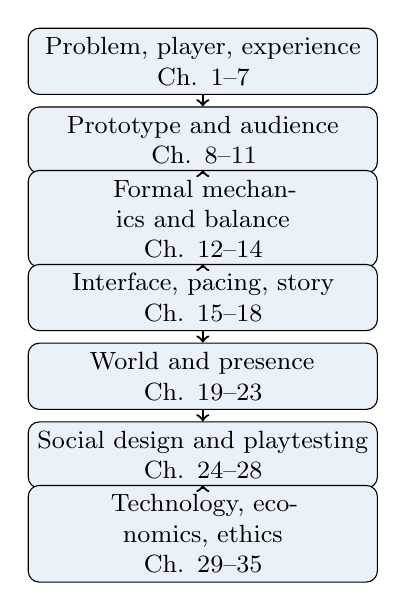
\begin{tikzpicture}[every node/.style={draw,rounded corners,fill=suitelight,text width=4.2cm,align=center,minimum height=0.6cm,font=\small},node distance=1.0cm]
\node (a) {Problem, player, experience\\Ch. 1--7};
\node (b) [below of=a] {Prototype and audience\\Ch. 8--11};
\node (c) [below of=b] {Formal mechanics and balance\\Ch. 12--14};
\node (d) [below of=c] {Interface, pacing, story\\Ch. 15--18};
\node (e) [below of=d] {World and presence\\Ch. 19--23};
\node (f) [below of=e] {Social design and playtesting\\Ch. 24--28};
\node (g) [below of=f] {Technology, economics, ethics\\Ch. 29--35};
\foreach \i/\j in {a/b,b/c,c/d,d/e,e/f,f/g} \draw[->,thick] (\i)--(\j);
\end{tikzpicture}\end{center}
Read chapter 8 early when beginning a prototype, and use chapter 28 playtesting methods continuously rather than postponing observation until Phase 6. The diagram represents a learning progression, not a claim that the book recommends a strict ordering beyond its chapter order.


\section{Phase 1: Foundations and experiential design}
Recommended preparation: basic observational reasoning.

\begin{longtable}{@{}p{0.11\linewidth}p{0.53\linewidth}p{0.28\linewidth}@{}}\toprule Chapter & Focus & Deliverable \\ \midrule\endhead
1 & In the Beginning, There Is the Designer & Interview notes \\
2 & The Designer Creates an Experience & Experience statement and two falsifiable experience claims. \\
3 & The Experience Takes Place in a Venue & Venue comparison and justified target-venue decision. \\
4 & The Experience Rises Out of a Game & Playable rule sheet and a falsifiable engagement hypothesis. \\
5 & The Game Consists of Elements & Elemental tetrad diagram plus change-impact table. \\
6 & The Elements Support a Theme & Theme statement \\
7 & The Game Begins with an Idea & Divergent idea log \\
\bottomrule\end{longtable}
Gate: submit a playable or inspectable artifact, a link to its evidence, one falsified or revised assumption, an accessibility consideration, and a reviewer decision (advance / revise / stop).


\section{Phase 2: Iterative design and audience}
Recommended preparation: paper prototyping and interview fundamentals.

\begin{longtable}{@{}p{0.11\linewidth}p{0.53\linewidth}p{0.28\linewidth}@{}}\toprule Chapter & Focus & Deliverable \\ \midrule\endhead
8 & The Game Improves through Iteration & Risk ledger \\
9 & The Game Is Made for a Player & Persona evidence map and audience acceptance criteria. \\
10 & The Experience Is in the Player's Mind & Mental-model diagram \\
11 & The Player's Mind Is Driven by the Player's Motivation & Motivation map and ethical rewards assessment. \\
\bottomrule\end{longtable}
Gate: submit a playable or inspectable artifact, a link to its evidence, one falsified or revised assumption, an accessibility consideration, and a reviewer decision (advance / revise / stop).


\section{Phase 3: Mechanics, probability, and balancing}
Recommended preparation: discrete mathematics, probability, deterministic programming.

\begin{longtable}{@{}p{0.11\linewidth}p{0.53\linewidth}p{0.28\linewidth}@{}}\toprule Chapter & Focus & Deliverable \\ \midrule\endhead
12 & Some Elements Are Game Mechanics & Mechanics specification \\
13 & Game Mechanics Must Be in Balance & Balance workbook \\
14 & Game Mechanics Support Puzzles & State graph \\
\bottomrule\end{longtable}
Gate: submit a playable or inspectable artifact, a link to its evidence, one falsified or revised assumption, an accessibility consideration, and a reviewer decision (advance / revise / stop).


\section{Phase 4: Interfaces, pacing, and narrative}
Recommended preparation: UI prototyping and directed graphs.

\begin{longtable}{@{}p{0.11\linewidth}p{0.53\linewidth}p{0.28\linewidth}@{}}\toprule Chapter & Focus & Deliverable \\ \midrule\endhead
15 & Players Play Games through an Interface & Interaction specification and usability test report. \\
16 & Experiences Can Be Judged by Their Interest Curves & Interest curve \\
17 & One Kind of Experience Is the Story & Narrative graph \\
18 & Story and Game Structures Can Be Artfully Merged with Indirect Control & Indirect-control design and observation record. \\
\bottomrule\end{longtable}
Gate: submit a playable or inspectable artifact, a link to its evidence, one falsified or revised assumption, an accessibility consideration, and a reviewer decision (advance / revise / stop).


\section{Phase 5: Worlds, characters, and presence}
Recommended preparation: spatial graphs, art critique, hardware constraints.

\begin{longtable}{@{}p{0.11\linewidth}p{0.53\linewidth}p{0.28\linewidth}@{}}\toprule Chapter & Focus & Deliverable \\ \midrule\endhead
19 & Stories and Games Take Place in Worlds & World rulebook and cross-medium consistency checklist. \\
20 & Worlds Contain Characters & Character graph \\
21 & Worlds Contain Spaces & Level plan \\
22 & Some Interfaces Create a Feeling of Presence & Presence audit with documented limitations and mitigation priorities. \\
23 & The Look and Feel of a World Is Defined by Its Aesthetics & Art direction specification and asset validation checklist. \\
\bottomrule\end{longtable}
Gate: submit a playable or inspectable artifact, a link to its evidence, one falsified or revised assumption, an accessibility consideration, and a reviewer decision (advance / revise / stop).


\section{Phase 6: Multiplayer, teams, and evidence}
Recommended preparation: collaboration, event logging, basic data ethics.

\begin{longtable}{@{}p{0.11\linewidth}p{0.53\linewidth}p{0.28\linewidth}@{}}\toprule Chapter & Focus & Deliverable \\ \midrule\endhead
24 & Some Games Are Played with Other Players & Multiplayer interaction rules and communication protocol sketch. \\
25 & Other Players Sometimes Form Communities & Community design assessment and trust-and-safety controls. \\
26 & The Designer Usually Works with a Team & Review minutes \\
27 & The Team Sometimes Communicates through Documents & Design document \\
28 & Good Games Are Created through Playtesting & Session plan \\
\bottomrule\end{longtable}
Gate: submit a playable or inspectable artifact, a link to its evidence, one falsified or revised assumption, an accessibility consideration, and a reviewer decision (advance / revise / stop).


\section{Phase 7: Technology, business, and responsibility}
Recommended preparation: performance profiling, software delivery and business analysis.

\begin{longtable}{@{}p{0.11\linewidth}p{0.53\linewidth}p{0.28\linewidth}@{}}\toprule Chapter & Focus & Deliverable \\ \midrule\endhead
29 & The Team Builds a Game with Technology & Technology evaluation matrix and architecture decision record. \\
30 & Your Game Will Probably Have a Client & Client needs interview \\
31 & The Designer Gives the Client a Pitch & Pitch deck outline \\
32 & The Designer and Client Want the Game to Make a Profit & Business model brief \\
33 & Games Transform Their Players & Transformation hypothesis \\
34 & Designers Have Certain Responsibilities & Ethical impact register and responsible-design decision. \\
35 & Each Designer Has a Purpose & Design manifesto \\
\bottomrule\end{longtable}
Gate: submit a playable or inspectable artifact, a link to its evidence, one falsified or revised assumption, an accessibility consideration, and a reviewer decision (advance / revise / stop).


\section{Capstone: playable vertical slice}
\begin{enumerate}
\item Write a one-page experience brief and player hypothesis.
\item Specify a core gameplay loop and formal mechanics state model.
\item Implement a playable prototype with deterministic debug/replay support.
\item Balance one consequential mechanic using controlled simulation.
\item Document runtime architecture, risks, and instrumentation consent.
\item Conduct two playtest rounds with an intentional design change.
\item Present a traceability matrix from experience goals to tests and observations.
\end{enumerate}

\section{Exit criteria}
\begin{itemize}
\item Every mechanics requirement has a test or explicit exception.
\item Every player-experience claim cites observation or is labeled unverified.
\item The prototype can be rebuilt from documented dependencies and commands.
\item Playtest documentation records recruitment, consent, limitations, and negative findings.
\item The final review includes accessible alternatives, privacy choices, and credible failure modes.
\end{itemize}

\end{document}
